%\documentclass[a4paper,10pt]{article}
\documentclass[10pt]{scrartcl}
%\usepackage[IL2]{fontenc}
\usepackage[utf8x]{inputenc}
\usepackage[czech]{babel}
\usepackage{listings}  
\usepackage{amsfonts,amsmath,amssymb,graphicx,color}
%\usepackage[total={17cm,27cm}, top=2cm, left=2cm, includefoot]{geometry}
%\usepackage{fancyhdr}
\usepackage{fkssugar}
\usepackage{hyperref}
\usepackage{mhchem}

%\usepackage{caption}

%  Umožňuje rozdělovat obsah na více sloupců
\usepackage{multicol}
\usepackage{booktabs}
\usepackage{pgffor}


% FJFI Types of popi
\renewcommand{\popi}[2]{$\frac{#1}{[\jd{#2}]}$}

\renewcommand{\figurename}{Obr.}
\addto\captionsczech{\renewcommand{\figurename}{Obr.}}
\addto\captionsczech{\renewcommand{\tablename}{Tab.}}
\def\mean#1{\left< #1 \right>}


\newcommand{\MakeFJFIHead}{
\setlength{\parindent}{0cm}
\begin{multicols}{2}
\textsf{\textbf{\FJFISubject \hspace{6.25cm} \FJFIInstitute}\\
\textbf{\large{\FJFITitle}}}

\begin{tabular}{rlrl}
	 \textsf{Jméno:} & \textbf{\textsf\FJFIAuthor}    &      \textsf{Kolega:} & \textsf{\FJFICoauthor} \\[1.5pt]
	  \textsf{Kruh:} & \textbf{\textsf\FJFIGroup}     & \textsf{Číslo skup.:} & \textsf{\FJFICircle}   \\[1.5pt]
	\textsf{Měřeno:} & \textbf{\textsf{\FJFILabdate}} &  \textsf{Zpracování}: & \textsf{\FJFIWorktime}
\end{tabular}

\begin{flushright}


\includegraphics[scale=0.2]{../img/fjfi.pdf}
%\hspace{0.4cm}
%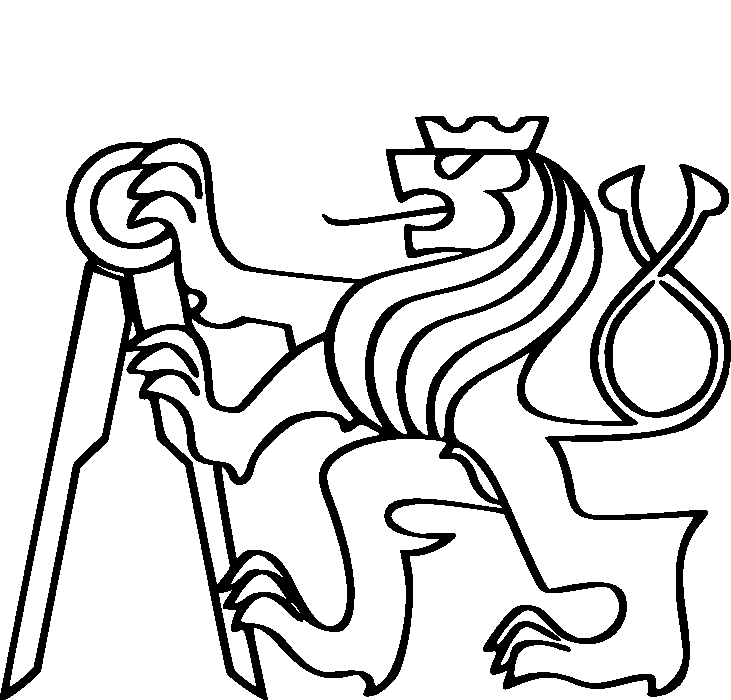
\includegraphics[scale=0.2]{../img/cvut.pdf}


\textsf{Klasifikace:} \hspace{3.2cm} 

\end{flushright}
\end{multicols}

\hrule
}




%  Nastaví autora, název, datum, skupinu měření apod. 
\newcommand{\Institute}{FJFI~ČVUT~v~Praze}
%\newcommand{\Subject}{Základy fyzikálních měření}
\newcommand{\Subject}{Fyzikální praktikum II}  %odkomentujte dle potřeby

%  Máte-li více spoluměřících než jednoho, vložte jen jejich příjmení
\newcommand{\Author}{Michal Červeňák}
\newcommand{\Coauthor}{Ondrej Glac} 
\newcommand{\Group}{Útorok} %den, kdy chodíte na praktika, nikoli obor
\newcommand{\Circle}{1} %číslo skupiny v rámci praktika, nikoli kruh

%  Tato část bude v každém protokolu jiná, nezapomeňte upravit!
\newcommand{\Title}{}
\newcommand{\Labdate}{28.2.2017} %datum měření, nikoli datum odevzdání
\newcommand{\Worktime}{\infy h} %jak dlouho vám trvalo vypracování protokolu


\begin{document}

\MakeFJFIHead{}

\section{Pracovní úkol}
\begin{enumerate}
\item DU: Odvo ďte vzorec (1) pro Brewsterův úhel úplné polarizace. Vycházejte z Obr. 1 a ze zákona lomu světla na rozhraní dvou optických prostředí. Spočtěte
Brewsterův úhel pro rozhraní vzduch - skleněné zrcadlo. Při měření Brewsterova
úhlu se doporučuje mít připravenou tabulku v Excelu pro výpočet stupně polarizace.
\item Při polarizaci bílého světla odrazem na černé skleněné desce proměřte závislost stupně polarizace
na sklonu desky a určete optimální hodnotu Brewsterova úhlu. Výsledky zaneste do grafu
a porovnejte s vypočtenou hodnotou z domácího úkolu.
\item Cernou otočnou desku nahraďte polarizačním filtrem a proměřte závislost intenzity polarizo-vaného světla na úhlu otočení analyzátoru (Malusův zákon). Výsledek srovnejte s teoretickou
předpovědí, znázorněte graficky a výsledek diskutujte.
\item Na optické lavici prozkoumejte vliv čtyř celofánových dvojlomných filtrů, způsobujících interferenci.
Vyzkoušejte vliv otáčení analyzátoru vůči polarizátoru a vliv otáčení dvojlomného filtru
mezi zkříženými i rovnoběžnými polarizátory v bílém světle. Pozorováním zjistěte, které vlnové
délky (barvy) se interferencí zvýrazní. Výsledky pozorování popište.
\item Pomocí dvou polarizačních filtrů, fotočlánku a barevných filtrů změřte měrnou otáčivost
křemene s tloušťkou 1 mm pro 4 vlnové délky světla. Jakou závislost pozorujete mezi vlnovou
délkou světla a měrnou otáčivostí? Naměřené hodnoty porovnejte s tabulkovými. Jak se změní
výsledek když použijete křemenný vzorek s větší tloušťkou? Diskutujte naměřené výsledky.
\end{enumerate}



\section{Teória}
Cievkou s $n_1$ závitami navinutej na toroide o polomere $r$, prechádza prúd $I_M$ 
Potom pre túto cievku môžeme intenzitu magnetického poľa $H$ vyjadriť ako
\eq{
H=\frac{n_1 I_M}{2\pi r}\,. \lbl{R_1}
}

Pre zmenu magnetickej indukcie $B$ v závislosti na výchylke balistického galvanometru $s$ platí vzťah 
\eq{
\Delta B = \frac{B K_b \lambda s_1^{*}}{n_2 S} \,, \lbl{R_2}
}
pričom $K_b$ je balistická konštanta, $R$ je odpor na odporovej dekáde, $s_1^{*}$ je výchylka galvanometra a $n_2$ počet meracích závitov. 

pre balistickú konštantu platí 
\eq{
R K_b \lambda = \frac{2L_{12} I_i}{s_1}\,,
}
kde $L_{12}$ je normálová cievka so známou indukčnosťou, a $s_1$ je výchylka pri zmene prúdu o $I_i$

%%%%%%%%%%%%%%%%%%%%%%%%%%%%%%%%%%%%%%%=
\subsubsection{Spracovanie chýb merania}

Označme $\mean{t}$ aritmetický priemer nameraných hodnôt $t_i$, a $\Delta t$ hodnotu $\mean{t}-t$, pričom 
\eq{
\mean{t} = \frac{1}{n}\sum_{i=1}^n t_i \,, \lbl{SCH_1}
}  
a chybu aritmetického priemeru 
\eq{
  \sigma_0=\sqrt{\frac{\sum_{i=1}^n \(t_i - \mean{t}\)^2}{n\(n-1\)}}\,, \lbl{SCH_2}
}
pričom $n$ je počet meraní.






\section{Pomôcky}
železná deska s magnetickými stojánky, \ce{He}-\ce{Ne} laser ($"633 nm"$, $"5 mW"$), 2 zrcadla na
stojánku, optická lavice s jezdci, 2 spojky ($+50$, $+200$), rozptylka ($−100$), sada kruhových otvorů,
nastavitelná štěrbina s mikrometrickým šroubem, stojan na mřížku, optická mřížka, stínítko na
zdi, stínítko, držák na stínítko a kruhové otvory, pásmové měřidlo ($5 m$), pravítko $"20 cm"$ a $"30 cm"$,
měřicí mikroskop, Abbeho kostka, rovinné zrcadlo s mikrometrickým šroubem, rovinné zrcadlo,
provázek.

\section{Postup merania}
\begin{enumerate}
\item Najskôr bol laserový zväzok pomocou kreplerového ďalekohľadu fokusovaný
\item do dráhy bolo umiestnené tienikom s difrakčnou dierkou
\item pomocou dvoch zrkadiel bol zväzok predlžený a nasmerovaný na stenu
\item pre jednotlivé diery boli obkreslené polohy maxím na papier
\item tienitko s dierami bolo vymenené za mriežku, zväzok bol opäť predlžený a difrakčné obrazce pre 10 rôznych otvorení obkreslené a odčítaná a zaznamená veľkosť diery mikrometrickým šróbom.
\item štrbina bola vymenená za mriežku, zväzok v tomto prípade nebolo potrebné predlžovať a na papier bola zaznamená poloha 0 a 1 maxima.
\item aparatúra bola rozobratá a na optickej lavici bol zostavený Michelsonův interferometr
\item Pomocou interferometru bola nameraná vlnová dĺžka laseru
\item po nameraní boli všetky obrazce premerané a určene jednotlivé vzdialenosti maxím.
\end{enumerate}

\section{Výsledky merania}
\subsection{Šošovka \uv{+200}}

Pre spojku \uv{+200} boli hodnoty zaznamenané v Tab. \ref{T_1}.
Pomocou programu \LaTeX\footnote{balíček metapost, ktorý je súčasťou distribúcie texlive-full.}
boli graficky určené polohy ohniskových vzdialeností $f_i$ pre jednotlivé merania 
\eq[m]{
\vect f_1 &= "[20.30\pm0.05,16.88\pm0.05] cm" \,,\\
\vect f_2 &= "[-,-]"\,,\\
\vect f_3 &= "[18.13\pm0.05,18.55\pm0.05] cm" \,,\\
\vect f_4 &="[17.70\pm0.05,18.92\pm0.05] cm" \,,
}
pričom pre druhé meranie sa nepodarilo určiť priesečník.
Zo zvyšných troch bodov bolo vypočítané ťažisko $\vect f="[18.71\pm0.9,18.12\pm0.8] cm" $ a pomocou vzťahu \ref{SCH_1} určená smerodajná odchylka, z $\vect f$ bola určená $f_g ="184.1\pm11.1 mm"$.

Z tabuľky pomocou vzťahu \ref{SCH_1} a \ref{SCH_2} sa určili mohutnosť šošovky $f\_B="181.76\pm4.87 mm"$.

\begin{table}[h]
\begin{center}
\begin{tabular}{ |  c | c | c | c | c | c | }
\hline
\popi{s_1}{cm}& \popi{s_2}{cm} & \popi{s_z}{cm}& \popi{s_o}{cm} & \popi{f\_B}{mm} & \popi{f_g}{mm} \\
\hline
$"50.20\pm0.05"$ & $"71.50\pm0.05"$ & $"100.0\pm0.1"$ & $"20.0\pm0.1"$ & $"185.82\pm0.1"$ & $"185.8\pm18.0"$\\ 
$"62.70\pm0.05"$ & $"65.50\pm0.05"$ & $"100.0\pm0.1"$ & $"30.0\pm0.1"$ & $"174.68\pm0.1"$ & $"-"$\\ 
$"35.50\pm0.05"$ & $"74.20\pm0.05"$ & $"100.0\pm0.1"$ & $"10.0\pm0.1"$ & $"183.34\pm0.1"$ & $"183.4\pm2.1"$\\ 
$"42.10\pm0.05"$ & $"73.70\pm0.05"$ & $"100.0\pm0.1"$ & $"15.0\pm0.1"$ & $"183.13\pm0.1"$ & $"183.1\pm5.1"$\\ 
\hline
\end{tabular}
\caption{Namerané hodnoty pre spojku \uv{+200}, pričom $s_1$ a $s_2$ sú polohy šošovky na dráhe, $s_o$ je poloha tienidla na dráhe, $s_z$ je poloha o zdroja (predmetu) na dráhe, $f\_B$ je vypočítané ohnisko Besselovou metodóu podľa vzťahu \ref{R_1} a $f_g$ je ohnisko učené grafickou metódou.} \label{T_1}
\end{center}
\end{table}

\subsection{Mikroskopický objektív}

Namerané hodnoty sú zaznamenané v tabuľke Tab. \ref{T_2} a z hodnôt $f\_B$ vypočítané pomocou vzťahu \ref{SCH_1} a \ref{SCH_2} vypočítaná ohnisková vzdialenosť $f = "92.15\pm2.63 mm"$.
Ďalej bola určená poloha ohniskových rovín, 
zdroj svetla bol umiestnený na optickej lavici $s_z="\(93.0\pm0.5\) cm"$, 
objektív $s_o="\(87.8\pm0.1\) cm"$, teda $x="\(52\pm6\) mm"$.
\begin{table}[h]
\begin{center}
\begin{tabular}{ |  c | c | c | c | c |  }
\hline
\popi{s_1}{cm}& \popi{s_2}{cm} & \popi{s_z}{cm}& \popi{s_o}{cm} & \popi{f\_B}{mm} \\
\hline
$"47.50\pm0.05"$ & $"88.70\pm0.05"$ & $"93.0\pm0.5"$ & $"30.0\pm0.1"$ & $"90.1\pm0.6"$ \\ 
$"37.30\pm0.05"$ & $"88.60\pm0.05"$ & $"93.0\pm0.5"$ & $"20.0\pm0.1"$ & $"92.4\pm0.6"$ \\ 
$"27.40\pm0.05"$ & $"88.80\pm0.05"$ & $"93.0\pm0.5"$ & $"10.0\pm0.1"$ & $"93.9\pm0.6"$ \\ 

\hline
\end{tabular}
\caption{Namerané hodnoty pre mikroskopický objektív, pričom $s_1$ a $s_2$ sú polohy šošovky na dráhe, $s_o$ je poloha tienidla na dráhe, $s_z$ je poloha o zdroja (predmetu) na dráhe, $f\_B$ je vypočítané ohnisko Besselovou metódou podľa vzťahu \ref{R_1}.} \label{T_2}
\end{center}
\end{table}

\subsection{Ramsdenový objektív}
Namerané hodnoty sú zaznamenané v tabuľke Tab. \ref{T_3} a z hodnôt $f\_B$ vypočítané pomocou vzťahu \ref{SCH_1} a \ref{SCH_2} vypočítaná ohnisková vzdialenosť $f = "93.27\pm0.73 mm"$.

Ďalej bola určená poloha ohniskových rovín, zdroj svetla bol umiestnený na optickej lavici $s_z="\(93.0\pm0.5\) cm"$, objektív $s_o="\(81.7\pm0.1\) cm"$, teda $x="\(113\pm6\) mm"$.

\begin{table}[h]
\begin{center}
\begin{tabular}{ |  c | c | c | c | c |  }
\hline
\popi{s_1}{cm}& \popi{s_2}{cm} & \popi{s_z}{cm}& \popi{s_o}{cm} & \popi{f\_B}{mm} \\
\hline
$"74.40\pm0.05"$ & $"92.80\pm0.05"$ & $"93.0\pm0.5"$ & $"50.0\pm0.1"$ & $"87.8\pm0.6"$ \\ 
$"64.30\pm0.05"$ & $"92.90\pm0.05"$ & $"93.0\pm0.5"$ & $"40.0\pm0.1"$ & $"93.9\pm0.6"$ \\ 
$"54.30\pm0.05"$ & $"93.00\pm0.05"$ & $"93.0\pm0.5"$ & $"30.0\pm0.1"$ & $"98.0\pm0.6"$ \\ 

\hline
\end{tabular}
\caption{Namerané hodnoty pre Ramsdenový objektív, pričom $s_1$ a $s_2$ sú polohy šošovky na dráhe, $s_o$ je poloha tienidla na dráhe, $s_z$ je poloha o zdroja (predmetu) na dráhe, $f\_B$ je vypočítané ohnisko Besselovou metódou podľa vzťahu \ref{R_1} } \label{T_3}
\end{center}
\end{table}


\subsection{Lupa}
Zväčšenie lupy bolo priamou metódou, pričom referenčná stupnica bola umiestnená do vzdialenosti $l="\(25\pm1\) cm"$ a presnosť určenia počtu dielikov bol $"1 dielik" = "10 \%"$ určené na $Z_l=10\pm1$. 


\subsection{Ďalekohľad}
Zväčšenie ďalekohľadu sme určili na základne porovnania zorných uhlov , pričom sme videli jeden dielik v ďalekohľade ako 20 dielikov \uv{vzoru} teda zväčšenie je $Z = 20\pm1$.

\begin{figure}
\includegraphics{data/graph_a.eps}
\caption{Grafické riešenie čočkovej rovnice pre spojku, kde malé body sú priesečniky $\vect f_i , i\in \{1,3,4\}$, šedý veľký krúžok je zistené ohnisko, a čierny je predpokladané ohnisko, čiarkovanou čiarou je druhé meranie, ktoré sa nepretína.}  \label{G_1}
\end{figure}



\section{Diskusia}
Obecne najväčším probémom v pri tomto meraní boli otrasy zeme spôsobné ostatnými ľuďmi v miestnosti ale aj prechádzajúcimi tramvajámi a autami po ceste vedľa budovy.
Tieto otrasy spôsobovali najväčšie problém pri interferometre kde nebolo možné rozlíšiť otrasy od pohybu. Tento fakt je premietnutý aj do chyby počtu maxím v tabuľke \ref{T_4}.

Pri ostatných úlohách otrasy nevadili natoľko aby sme ich chybu museli zohľadňovať.

Pri určovaní urazenej dráhy laserového paprsku sme túto dráhu zmerali až po skončení experimentu a tým pádom sme uvažovali nepresnosť merania v podobe $"20 cm"$.

Pri meraní rozmerov pomocou miktroskopu, sme mali najväčší problém určiť, presnú hranu/okraj diery, rozhranie týchto dier nebolo ostré ale na mnohćh miestach zostrapené. Preto toto meranie je predovšetkým týmto faktom výrazne zaťažené. Teda pre malé otvory sa problematický určuje touto metódou ich rozmer. 

\section{Záver}

V tabuľkách Tab. \ref{T_1} a Tab. \ref{T_2} vidíme porovnanie nameraných veľkosti otvorov v porovnaní s vypočítanými hodnotami pomocou difrakcie.

Mriežková konštanta mriežky bola určená na
\eq{
d = "\(1.54\pm0.054\)\cdot10^{-6} m"\,.
}

Určili sme vlnovú dlžku použitého laseru viď vzťah \ref{R_V_4}.

\begin{thebibliography}{2}
\bibitem{C_1}
Interference a difrakce světla [cit. 16.5.2017]Dostupné po prihlásení z Kurz: Fyzikální praktikum II:\url{https://praktikum.fjfi.cvut.cz/pluginfile.php/423/mod_resource/content/8/10_interference_170218.pdf}




\end{thebibliography}

\end{document}

